\section{Results}
\label{sec:results}

In this section we analyze the created dataset, comparing it to the tickets we collected from the survey. \\
The final dataset of HR tickets automatically generated is composed by exactly 16,000 tickets, 2000 for each category. On the other hand, we collected 259 test tickets from 29 different respondents. \\
To evaluate the generation of the tickets, we have used a handful of traditional unsupervised text evaluation techniques. We were not able to exploit more complex classical metrics, such as BLEU and ROUGE, not having real data as references for each prompt.
The reported metrics are:
\begin{itemize}
    \item avg ttr unigram: average TTR(type token ratio) for the unigrams of the tickets\\ 
    \begin{equation*}
        TTR = \frac{number\_of\_unique\_unigrams}{total\_number\_of\_unigrams}
    \end{equation*}
    \item avg ttr bigram: average TTR(type token ratio) for the bigram of the tickets\\ 
    \begin{equation*}
        TTR = \frac{number\_of\_unique\_bigrams}{total\_number\_of\_bigrams}
    \end{equation*}
    \item avg ratios of nouns: average ratio of nouns in the tickets\\
    \begin{equation*}
        noun\_ratio = \frac{counter\_noun\_words}{counter\_all\_words}
    \end{equation*}
    \item avg ratios of verbs: average ratio of verbs in the tickets\\
    \begin{equation*}
        verb\_ratio = \frac{counter\_verb\_words}{counter\_all\_words}
    \end{equation*}
    \item avg\_word\_frequency: average frequency of words, using as frequency estimates a dump of the English version of Wikipedia, considering only words appearing at least 10 times\\
    \begin{equation*}
        word\_freq= 
        \begin{cases}
            log_{e}(word\_freq\_wiki),& \text{if } word\_freq\_wiki\geq 10\\
            skip,                   & \text{otherwise}
        \end{cases}
    \end{equation*}
\end{itemize}
First, we reported the type-token-rations given that high-quality writing has been associated with the presence of more diverse words and phrases\cite{pitler2008revisiting}. We computed them for each ticket and then we averaged the results. \\
Second, since lower frequency words indicate a more advanced output\cite{crossley2011development}, we compute the average word frequency of the generated words.\\
Then, we calculate nouns and verb ratios over sentence length, as indicators of syntactic complexity, and therefore richer text\cite{mcnamara2010linguistic}. To single out nouns and verbs, we use the pre-trained Spacy POS model. \\\\
We report in \autoref{table:initial_results} the results we obtained initially. The metrics have been calculated not only on the tickets generated by the model and the tickets of the surveys, but also on some baseline datasets (\textit{Amazon reviews}, \textit{Reddit comments} and \textit{NIPS papers}). The datasets have been chosen to be as diversified as possible in terms of text longevity, type of language and terms used. \\ %TODO: maybe add for each dataset a brief description
The main takeaways from the metrics are:
\begin{itemize}
    \item The model tends to write more unique words and not to repeat itself, since the average TTR of both unigrams and bigrams are higher in the tickets of the survey
    \item The model tends to use more nouns than a real person
    \item The model tends the same number of verbs as a real person
    \item The average number of words ( word count ) varies a lot from category to category, both in generated and survey tickets
\end{itemize}
We know that these analyses are not completely reliable due to the low number of real data compared to the size of our dataset. However they are a good indication of how to improve the generation. \\
For this reason, we changed the parameters of the ticket creation and recreated the dataset from scratch, in order to be more akin to the survey tickets. \\
The final results are shown in \autoref{table:final_results}. \\
Some of the surveys' metrics change a bit compared to the first table, this is due to some late respondents to the survey, which skewed a little bit the final test metrics.

\begin{table}[h]
    \resizebox{\textwidth}{!}{
    \setlength\extrarowheight{16pt}
    \begin{tabular}{|l|l|l|l|l|l|l|}
    \hline
    Dataset                                                                           & \shortstack{avg ttr\\unigram} & \shortstack{avg ttr\\bigram} & \shortstack{avg ratios\\of nouns} & \shortstack{avg ratios\\of verbs} & \shortstack{avg word\\frequency} & \shortstack{avg word\\count} \\ \hline
    Amazon reviews                                                                    & 0.81                          & 0.98                         & 0.16                              & 0.10                              & 13.86, $\sigma$=0.47               & 73.73, $\sigma$=71.75    \\ \hline
    Reddit comments                                                                   & 0.91                          & 0.99                         & 0.15                              & 0.11                              & 13.33, $\sigma$=1.53               & 37.70, $\sigma$=84.96    \\ \hline
    NIPS papers                                                                       & 0.26                          & 0.72                         & 0.18                              & 0.06                              & 13.50, $\sigma$=0.25               & 5798.40, $\sigma$=737.17 \\ \hline
    Tickets survey & 0.87                                                             & 0.99                          & 0.17                         & 0.11                              & 13.84                             & 42.73, $\sigma$=28.83                  \\ \hline
    Tickets generated by GPT                                                          & 0.93                          & 1.00                         & 0.14                              & 0.10                              & 13.84, $\sigma$=0.35               & 57.87, $\sigma$=19.13    \\ \hline
    \shortstack[l]{Survey\\Salary\_Salary raise}                                      & 0.85                          & 0.99                         & 0.20                              & 0.10                              & 13.85, $\sigma$=0.56              & \textcolor{red}{55.65}, $\sigma$=35.67    \\ \hline
    \shortstack[l]{GPT\\Salary\_Salary raise}                                         & 0.90                          & 1.00                         & 0.15                              & 0.10                              & 13.72, $\sigma$=0.33              & \textcolor{red}{70.73}, $\sigma$=16.36    \\ \hline
    \shortstack[l]{Survey\\Complaint\_Complaint}                                      & 0.83                          & 0.98                         & 0.15                              & 0.13                              & 13.66, $\sigma$=0.91              & 63.64, $\sigma$=46.67    \\ \hline
    \shortstack[l]{GPT\\Complaint\_Complaint}                                         & 0.91                          & 0.99                         & 0.14                              & 0.12                              & 13.94, $\sigma$=0.32              & 72.81, $\sigma$=21.62    \\ \hline
    \shortstack[l]{Survey\\Life event\_Personal issues}                               & 0.89                          & 0.99                         & 0.17                              & 0.12                              & 13.99, $\sigma$=0.56              & \textcolor{red}{33.54}, $\sigma$=19.85    \\ \hline
    \shortstack[l]{GPT\\Life event\_Personal issues}                                  & 0.92                          & 1.00                         & 0.13                              & 0.12                              & 14.08, $\sigma$=0.25              & \textcolor{red}{63.88}, $\sigma$=15.62    \\ \hline
    \shortstack[l]{Survey\\Refund\_Refund travel}                                     & 0.90                          & 0.99                         & 0.17                              & 0.11                              & 13.56, $\sigma$=0.56              & 34.76, $\sigma$=17.02    \\ \hline
    \shortstack[l]{GPT\\Refund\_Refund travel}                                        & 0.96                          & 1.00                         & 0.16                              & 0.08                              & 13.72, $\sigma$=0.38              & 38.91, $\sigma$=10.83    \\ \hline
    \shortstack[l]{Survey\\Timetable change\_Shift change}                            & 0.83                          & 0.99                         & 0.16                              & 0.10                              & 14.16, $\sigma$=0.66              & 38.15, $\sigma$=15.30    \\ \hline
    \shortstack[l]{GPT\\Timetable change\_Shift change}                               & 0.93                          & 1.00                         & 0.13                              & 0.10                              & 13.79, $\sigma$=0.37              & 47.95, $\sigma$=9.72     \\ \hline
    \shortstack[l]{Survey\\Ask information\_Accommodation}                            & 0.88                          & 0.99                         & 0.17                              & 0.11                              & 13.80, $\sigma$=0.50              & 39.93, $\sigma$=23.89    \\ \hline
    \shortstack[l]{GPT\\Ask information\_Accommodation}                               & 0.95                          & 1.00                         & 0.14                              & 0.10                              & 13.68, $\sigma$=0.36              & 47.10, $\sigma$=10.59    \\ \hline
    \shortstack[l]{Survey\\Life event\_Health issues}                                 & 0.90                          & 0.99                         & 0.17                              & 0.13                              & 13.88, $\sigma$=0.44              & \textcolor{red}{31.92}, $\sigma$=14.70    \\ \hline
    \shortstack[l]{GPT\\Life event\_Health issues}                                    & 0.91                          & 1.00                         & 0.14                              & 0.10                              & 13.84, $\sigma$=0.33              & \textcolor{red}{59.07}, $\sigma$=16.06    \\ \hline
    \shortstack[l]{Survey\\Salary\_Gender pay gap}                                    & 0.85                          & 0.97                         & 0.21                              & 0.11                              & 13.87, $\sigma$=0.43              & 53.94, $\sigma$=32.71    \\ \hline
    \shortstack[l]{GPT\\Salary\_Gender pay gap}                                       & 0.93                          & 0.99                         & 0.15                              & 0.11                              & 13.96, $\sigma$=0.28              & 62.52, $\sigma$=18.67    \\ \hline
    \end{tabular}}
    \caption{Initial Results}\label{table:initial_results}
\end{table}



\begin{table}[h]
    \resizebox{\textwidth}{!}{
    \setlength\extrarowheight{16pt}
    \begin{tabular}{|l|l|l|l|l|l|l|}
    \hline
    Dataset                                                                           & \shortstack{avg ttr\\unigram} & \shortstack{avg ttr\\bigram} & \shortstack{avg ratios\\of nouns} & \shortstack{avg ratios\\of verbs} & \shortstack{avg word\\frequency} & \shortstack{avg word\\count} \\ \hline
    Amazon reviews                                                                    & 0.81                          & 0.98                         & 0.16                              & 0.10                              & 13.86, $\sigma$=0.47               & 73.73, $\sigma$=71.75          \\ \hline
    Reddit comments                                                                   & 0.91                          & 0.99                         & 0.15                              & 0.11                              & 13.33, $\sigma$=1.53               & 37.70, $\sigma$=84.96          \\ \hline
    Tickets survey                                                                    & 0.86                          & 0.99                         & 0.17                              & 0.11                              & 13.89, $\sigma$=0.59               & 44.43, $\sigma$=27.46          \\ \hline
    Tickets generated by GPT                                                          & 0.94                          & 1.00                         & 0.14                              & 0.10                              & 13.86, $\sigma$=0.39               & 49.22, $\sigma$=15.49          \\ \hline
    \shortstack[l]{Survey\\Salary\_Salary raise}                                      & 0.84                          & 0.99                         & 0.21                              & 0.10                              & 13.89, $\sigma$=0.52               & 55.10, $\sigma$=32.44          \\ \hline
    \shortstack[l]{GPT\\Salary\_Salary raise}                                         & 0.90                          & 1.00                         & 0.15                              & 0.10                              & 13.73, $\sigma$=0.35               & 62.87, $\sigma$=14.12          \\ \hline
    \shortstack[l]{Survey\\Complaint\_Complaint}                                      & 0.82                          & 0.98                         & 0.15                              & 0.13                              & 13.74, $\sigma$=0.84               & 62.74, $\sigma$=42.83          \\ \hline
    \shortstack[l]{GPT\\Complaint\_Complaint}                                         & 0.92                          & 0.99                         & 0.14                              & 0.11                              & 13.94, $\sigma$=0.33               & 59.46, $\sigma$=18.39          \\ \hline
    \shortstack[l]{Survey\\Life event\_Personal issues}                               & 0.88                          & 0.99                         & 0.17                              & 0.12                              & 14.03, $\sigma$=0.55               & 38.15, $\sigma$=20.86          \\ \hline
    \shortstack[l]{GPT\\Life event\_Personal issues}                                  & 0.94                          & 1.00                         & 0.14                              & 0.11                              & 14.19, $\sigma$=0.30               & 45.49, $\sigma$=16.94          \\ \hline
    \shortstack[l]{Survey\\Refund\_Refund travel}                                     & 0.88                          & 0.99                         & 0.17                              & 0.11                              & 13.61, $\sigma$=0.53               & 37.50, $\sigma$=17.36          \\ \hline
    \shortstack[l]{GPT\\Refund\_Refund travel}                                        & 0.96                          & 1.00                         & 0.16                              & 0.08                              & 13.72, $\sigma$=0.38               & 39.52, $\sigma$=10.46          \\ \hline
    \shortstack[l]{Survey\\Timetable change\_Shift change}                            & 0.83                          & 0.99                         & 0.16                              & 0.10                              & 14.17, $\sigma$=0.62               & 38.73, $\sigma$=14.71          \\ \hline
    \shortstack[l]{GPT\\Timetable change\_Shift change}                               & 0.93                          & 1.00                         & 0.12                              & 0.10                              & 13.74, $\sigma$=0.40               & 42.80, $\sigma$=7.55           \\ \hline
    \shortstack[l]{Survey\\Ask information\_Accommodation}                            & 0.87                          & 0.99                         & 0.16                              & 0.11                              & 13.90, $\sigma$=0.50               & 41.86, $\sigma$=23.79          \\ \hline
    \shortstack[l]{GPT\\Ask information\_Accommodation}                               & 0.95                          & 1.00                         & 0.14                              & 0.10                              & 13.65, $\sigma$=0.38               & 46.79, $\sigma$=10.99          \\ \hline
    \shortstack[l]{Survey\\Life event\_Health issues}                                 & 0.87                          & 0.99                         & 0.17                              & 0.13                              & 13.94, $\sigma$=0.42               & 37.91, $\sigma$=21.80          \\ \hline
    \shortstack[l]{GPT\\Life event\_Health issues}                                    & 0.94                          & 1.00                         & 0.16                              & 0.09                              & 13.95, $\sigma$=0.37               & 43.36, $\sigma$=11.26          \\ \hline
    \shortstack[l]{Survey\\Salary\_Gender pay gap}                                    & 0.85                          & 0.97                         & 0.22                              & 0.11                              & 13.87, $\sigma$=0.41               & 53.14, $\sigma$=31.13          \\ \hline
    \shortstack[l]{GPT\\Salary\_Gender pay gap}                                       & 0.94                          & 1.00                         & 0.14                              & 0.11                              & 13.99, $\sigma$=0.29               & 53.49, $\sigma$=13.51          \\ \hline
    \end{tabular}}
    \caption{Final Results}\label{table:final_results}
\end{table}

% TODO: add self-bleu 

\subsection*{Topic analysis}
Topic modeling is a type of statistical modeling technique used to discover the hidden topics and patterns in a corpus of text. It is a type of unsupervised machine learning method that automatically discovers topics from a collection of documents by analyzing words and phrases in each document. Topics are usually represented by word clusters or distributions that are related to each other. Topic modeling can be used to generate meaningful summaries about large collections of documents. \\
We used topic modeling to visualize in a summarized form the major topics of our dataset and to verify that the topics created correspond to the ones in the taxonomy.\todo[inline]{one could ask how the topic analysis on the manually-produced dataset relates to the generated one, what are similarities/differences etc. The reason is clearly stated but the question may arise, if you have the data, it might be worth including some words on this aspect.} \\
The model of topic modeling we chose is BERTopic\cite{grootendorst2022bertopic}. BERTopic generates document embedding with pre-trained transformer-based language models, clusters these embeddings, and finally, generates topic representations with the class-based Term Frequency-Inverse Document Frequency (TF-IDF)\todo[inline]{Term Frequency-Inverse Document Frequency (TF-IDF)} procedure
\begin{algorithm}
    \caption*{BERTopic}
    \begin{algorithmic}[1]
      \State Documents are embedded to create representations in vector space using Sentence-BERT
      \State The embeddings generated are reduced in dimensionality using UMAP
      \State The reduced embeddings are clustering used HDBSCAN. HDBSCAN is a variation of the hierarchical clustering algorithm DBSCAN that models clusters using a soft-clustering approach, allowing noise to be modeled as outliers
      \State The most relevant terms for each topic are found using a class-based version of TF-IDF. All documents in a cluster are treated as a single document by simply concatenating them, so we measure how much information a term provides to a class instead of a document.
      \State If the user requests a number of topics smaller than the number of topics generated, the least common topics are iteratively merged with their most similar topic, until the number of topics requested is satisfied.
    \end{algorithmic}
\end{algorithm}

The formula of the class-based TF-IDF is:
\begin{equation*}
    W_{t,c} = tf_{t,c} \cdot \log(1 + \frac{A}{tf_{t}})
\end{equation*}
where $tf_{t,c}$ is the frequency of term $t$ in class $c$, $A$ is the average number of words per class and $tf_{t}$ is the frequency of term $t$ across all classes.

In \autoref{fig:hierarchical_topicmodel} we show all the topics that BERTopic outputs, and in \autoref{fig:barchart_topicmodel} the grouped major 8 topics. \\
We are satisfied with the results, we can clearly recognize 7 of our 8 categories in the topics created, the only one missing is the request of time off due to personal reasons, that have been incorporated in Topic 3. \\
The topics generated by BERTopic are:
\begin{itemize}
    \item \textbf{Topic 0}: Request of shift change
    \item \textbf{Topic 1}: Request of explanation of wage gap between genders
    \item \textbf{Topic 2}: Official complaint about colleague/superior
    \item \textbf{Topic 3}: Request of time off due to health reasons
    \item \textbf{Topic 4}: Request of salary increase
    \item \textbf{Topic 5}: Request of refund for work travel
    \item \textbf{Topic 6}: Request of refund for work travel
    \item \textbf{Topic 7}: Request of information for new accommodation
\end{itemize}


\begin{figure}[h] 
    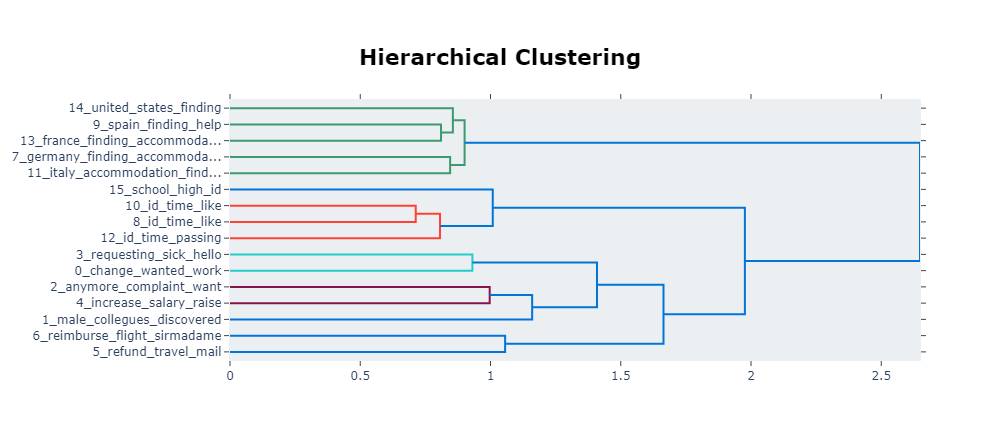
\includegraphics[width=\textwidth]{images/hierarchy_topic_model.png}
    \caption{Hierarchy of all topics generated by BERTopic}
    \label{fig:hierarchical_topicmodel}
\end{figure}


\begin{figure}[h] 
    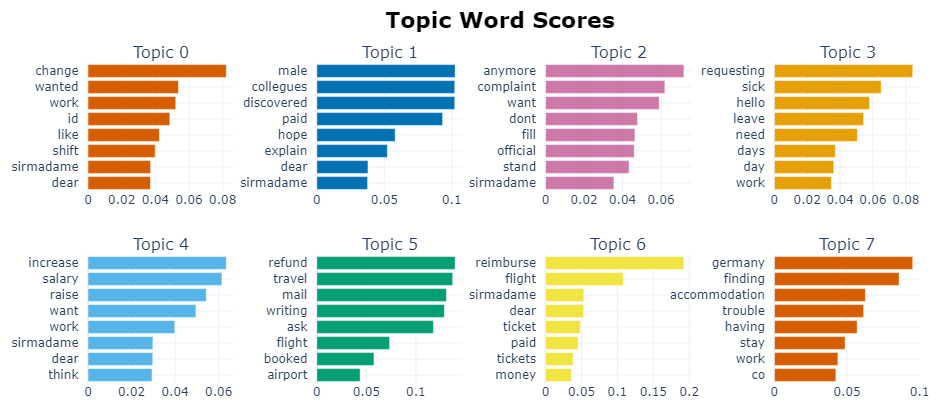
\includegraphics[width=\textwidth]{images/barchart_topicmodel.png}
    \caption{Main 8 topics generated by BERTopic}
    \label{fig:barchart_topicmodel}
\end{figure}    
